\begin{enumerate}[label=\thesection.\arabic*,ref=\thesection.\theenumi]
\numberwithin{equation}{enumi}
\numberwithin{figure}{enumi}
\numberwithin{table}{enumi}
\item If $\overrightarrow {a}$ is a nonzero vector of magnitude 'a' and $\lambda$ a nonzero scalar , then $\lambda\overrightarrow {a}$ is unit vector if
\begin{enumerate} 
\item $\lambda=1$ 
\item $\lambda=-1$
\item $a=\abs{\lambda}$
\item $a=1/\abs{\lambda}$  
\end{enumerate}
\item Compute the magnitude of the following vectors:
\begin{align*}
\vec{a}=\hat{i}+\hat{j}+k; \vec{b}=2\hat{i}-7\hat{j}-3\hat{k}; \vec{c}=\frac{1}{\sqrt{3}}\hat{i}+\frac{1}{\sqrt{3}}\hat{j}-\frac{1}{3}\hat{k}
\end{align*}
    \solution 
		\iffalse
\documentclass[12pt]{article}
\usepackage{graphicx}
%\documentclass[journal,12pt,twocolumn]{IEEEtran}
\usepackage[none]{hyphenat}
\usepackage{graphicx}
\usepackage{listings}
\usepackage[english]{babel}
\usepackage{graphicx}
\usepackage{caption} 
\usepackage{hyperref}
\usepackage{booktabs}
\usepackage{commath}
\usepackage{gensymb}
\usepackage{array}
\usepackage{amsmath}   % for having text in math mode
\usepackage{listings}
\lstset{
  frame=single,
  breaklines=true
}
  
%Following 2 lines were added to remove the blank page at the beginning
\usepackage{atbegshi}% http://ctan.org/pkg/atbegshi
\AtBeginDocument{\AtBeginShipoutNext{\AtBeginShipoutDiscard}}
%


%New macro definitions
\newcommand{\mydet}[1]{\ensuremath{\begin{vmatrix}#1\end{vmatrix}}}
\providecommand{\brak}[1]{\ensuremath{\left(#1\right)}}
\providecommand{\norm}[1]{\left\lVert#1\right\rVert}
\newcommand{\solution}{\noindent \textbf{Solution: }}
\newcommand{\myvec}[1]{\ensuremath{\begin{pmatrix}#1\end{pmatrix}}}
\let\vec\mathbf


\begin{document}
\begin{center}
\title{\textbf{Vectors}}
\date{\vspace{-5ex}} %Not to print date automatically
\maketitle
\end{center}
\setcounter{page}{1}
\section*{12$^{th}$ Maths - Exercise 10.2.1}

\begin{enumerate}
\item Compute the magnitude of the following vectors 
$\\ \overrightarrow{a}=\hat{i}+\hat{j}+\hat{k},\overrightarrow{b}=2\hat{i}-7\hat{j}+3\hat{k}$ and $\overrightarrow{c}=\dfrac{1}{\sqrt{3}}\hat{i}+\dfrac{1}{\sqrt{3}}\hat{j}-\dfrac{1}{\sqrt{3}}\hat{k}$.\\
\solution
\fi
Let 
\begin{align}
 \vec{a} = \myvec{1\\1\\1} , \vec{b} = \myvec{2\\ -7 \\ 3},\vec{c} = \myvec{\dfrac{1}{\sqrt{3}}\\ \dfrac{1}{\sqrt{3}} \\ -\dfrac{1}{\sqrt{3}}} 
\label{eq:chapters/12/10/2/1/1}
\end{align}
Then
\begin{align}
	\norm{\vec{a}}&=\sqrt{\vec{a}}^{\top}\vec{a}=\norm{\vec{a}}=\sqrt{3}, 
	\label{eq:chapters/12/10/2/1/3}
	\\ \norm{\vec{b}}&=\sqrt{\vec{b}}^{\top}\vec{b}=\norm{\vec{b}}= \sqrt{62}, 
	\label{eq:chapters/12/10/2/1/4}
	\\ \norm{\vec{c}}&=\sqrt{\vec{c}}^{\top}\vec{c}	=
\norm{\vec{c}}=1
	\label{eq:chapters/12/10/2/1/5}
\end{align}




\item Find the unit vector in the direction of the vector $\vec{a}=\hat{i}+\hat{j}+2\hat{k}$.
\item Find the unit vector in the direction of vector $\overrightarrow{PQ}$ , where $\vec{P}$ and $\vec{Q}$ are the points
(1, 2, 3) and (4, 5, 6), respectively.
\item For given vectors, $\vec{a}=2\hat{i}-\hat{j}+2\hat{k}$ and $\vec{b}=-\hat{i}+\hat{j}-\hat{k}$ , find the unit vector in the
direction of the vector $\vec{a}+\vec{b}$.
\\
    \solution 
		\iffalse
\documentclass[journal,12pt,twocolumn]{IEEEtran}
%
\usepackage{setspace}
\usepackage{gensymb}
%\doublespacing
\singlespacing

%\usepackage{graphicx}
%\usepackage{amssymb}
%\usepackage{relsize}
\usepackage[cmex10]{amsmath}
%\usepackage{amsthm}
%\interdisplaylinepenalty=2500
%\savesymbol{iint}
%\usepackage{txfonts}
%\restoresymbol{TXF}{iint}
%\usepackage{wasysym}
\usepackage{amsthm}
%\usepackage{iithtlc}
\usepackage{mathrsfs}
\usepackage{txfonts}
\usepackage{stfloats}
\usepackage{bm}
\usepackage{cite}
\usepackage{cases}
\usepackage{subfig}
%\usepackage{xtab}
\usepackage{longtable}
\usepackage{multirow}
%\usepackage{algorithm}
%\usepackage{algpseudocode}
\usepackage{enumitem}
\usepackage{mathtools}
\usepackage{steinmetz}
\usepackage{tikz}
\usepackage{circuitikz}
\usepackage{verbatim}
\usepackage{tfrupee}
\usepackage[breaklinks=true]{hyperref}
%\usepackage{stmaryrd}
\usepackage{tkz-euclide} % loads  TikZ and tkz-base
%\usetkzobj{all}
\usetikzlibrary{calc,math}
\usepackage{listings}
    \usepackage{color}                                            %%
    \usepackage{array}                                            %%
    \usepackage{longtable}                                        %%
    \usepackage{calc}                                             %%
    \usepackage{multirow}                                         %%
    \usepackage{hhline}                                           %%
    \usepackage{ifthen}                                           %%
  %optionally (for landscape tables embedded in another document): %%
    \usepackage{lscape}     
\usepackage{multicol}
\usepackage{chngcntr}
%\usepackage{enumerate}

%\usepackage{wasysym}
%\newcounter{MYtempeqncnt}
\DeclareMathOperator*{\Res}{Res}
%\renewcommand{\baselinestretch}{2}
\renewcommand\thesection{\arabic{section}}
\renewcommand\thesubsection{\thesection.\arabic{subsection}}
\renewcommand\thesubsubsection{\thesubsection.\arabic{subsubsection}}

\renewcommand\thesectiondis{\arabic{section}}
\renewcommand\thesubsectiondis{\thesectiondis.\arabic{subsection}}
\renewcommand\thesubsubsectiondis{\thesubsectiondis.\arabic{subsubsection}}

% correct bad hyphenation here
\hyphenation{op-tical net-works semi-conduc-tor}
\def\inputGnumericTable{}                                 %%

\lstset{
%language=C,
frame=single, 
breaklines=true,
columns=fullflexible
}
%\lstset{
%language=tex,
%frame=single, 
%breaklines=true
%}

\begin{document}
%


\newtheorem{theorem}{Theorem}[section]
\newtheorem{problem}{Problem}
\newtheorem{proposition}{Proposition}[section]
\newtheorem{lemma}{Lemma}[section]
\newtheorem{corollary}[theorem]{Corollary}
\newtheorem{example}{Example}[section]
\newtheorem{definition}[problem]{Definition}
%\newtheorem{thm}{Theorem}[section] 
%\newtheorem{defn}[thm]{Definition}
%\newtheorem{algorithm}{Algorithm}[section]
%\newtheorem{cor}{Corollary}
\newcommand{\BEQA}{\begin{eqnarray}}
\newcommand{\EEQA}{\end{eqnarray}}
\newcommand{\define}{\stackrel{\triangle}{=}}

\bibliographystyle{IEEEtran}
%\bibliographystyle{ieeetr}


\providecommand{\mbf}{\mathbf}
\providecommand{\pr}[1]{\ensuremath{\Pr\left(#1\right)}}
\providecommand{\qfunc}[1]{\ensuremath{Q\left(#1\right)}}
\providecommand{\sbrak}[1]{\ensuremath{{}\left[#1\right]}}
\providecommand{\lsbrak}[1]{\ensuremath{{}\left[#1\right.}}
\providecommand{\rsbrak}[1]{\ensuremath{{}\left.#1\right]}}
\providecommand{\brak}[1]{\ensuremath{\left(#1\right)}}
\providecommand{\lbrak}[1]{\ensuremath{\left(#1\right.}}
\providecommand{\rbrak}[1]{\ensuremath{\left.#1\right)}}
\providecommand{\cbrak}[1]{\ensuremath{\left\{#1\right\}}}
\providecommand{\lcbrak}[1]{\ensuremath{\left\{#1\right.}}
\providecommand{\rcbrak}[1]{\ensuremath{\left.#1\right\}}}
\theoremstyle{remark}
\newtheorem{rem}{Remark}
\newcommand{\sgn}{\mathop{\mathrm{sgn}}}
\providecommand{\abs}[1]{\left\vert#1\right\vert}
\providecommand{\res}[1]{\Res\displaylimits_{#1}} 
\providecommand{\norm}[1]{\left\lVert#1\right\rVert}
%\providecommand{\norm}[1]{\lVert#1\rVert}
\providecommand{\mtx}[1]{\mathbf{#1}}
\providecommand{\mean}[1]{E\left[ #1 \right]}
\providecommand{\fourier}{\overset{\mathcal{F}}{ \rightleftharpoons}}
%\providecommand{\hilbert}{\overset{\mathcal{H}}{ \rightleftharpoons}}
\providecommand{\system}{\overset{\mathcal{H}}{ \longleftrightarrow}}
	%\newcommand{\solution}[2]{\textbf{Solution:}{#1}}
\newcommand{\solution}{\noindent \textbf{Solution: }}
\newcommand{\cosec}{\,\text{cosec}\,}
\providecommand{\dec}[2]{\ensuremath{\overset{#1}{\underset{#2}{\gtrless}}}}
\newcommand{\myvec}[1]{\ensuremath{\begin{pmatrix}#1\end{pmatrix}}}
\newcommand{\mydet}[1]{\ensuremath{\begin{vmatrix}#1\end{vmatrix}}}
%\numberwithin{equation}{section}
\numberwithin{equation}{subsection}
%\numberwithin{problem}{section}
%\numberwithin{definition}{section}
\makeatletter
\@addtoreset{figure}{problem}
\makeatother

\let\StandardTheFigure\thefigure
\let\vec\mathbf
%\renewcommand{\thefigure}{\theproblem.\arabic{figure}}
\renewcommand{\thefigure}{\theproblem}
%\setlist[enumerate,1]{before=\renewcommand\theequation{\theenumi.\arabic{equation}}
%\counterwithin{equation}{enumi}


%\renewcommand{\theequation}{\arabic{subsection}.\arabic{equation}}

\def\putbox#1#2#3{\makebox[0in][l]{\makebox[#1][l]{}\raisebox{\baselineskip}[0in][0in]{\raisebox{#2}[0in][0in]{#3}}}}
     \def\rightbox#1{\makebox[0in][r]{#1}}
     \def\centbox#1{\makebox[0in]{#1}}
     \def\topbox#1{\raisebox{-\baselineskip}[0in][0in]{#1}}
     \def\midbox#1{\raisebox{-0.5\baselineskip}[0in][0in]{#1}}

\vspace{3cm}


\title{EE2802: Assignment5}
\author{Nikam Pratik Balasaheb (EE21BTECH11037)}





% make the title area
\maketitle

\newpage

%\tableofcontents

\bigskip

\renewcommand{\thefigure}{\theenumi}
\renewcommand{\thetable}{\theenumi}
%\renewcommand{\theequation}{\theenumi}

\section{Problem}
For the vectors $ \vec a = \myvec{ 2\\-1\\2 } \text{ and } \vec b = \myvec{ -1\\1\\-1 }$, find the unit vector along the direction of $ \vec a + \vec b$.

\section{Solution}
\fi
Since
\begin{align}
\vec a + \vec b = \vec u = \myvec{ 2\\-1\\2 } + \myvec{ -1\\1\\-1 }
= \myvec{ 1\\0\\1 }
\end{align}
the unit vector in direction of $\vec u$ is,
\begin{align}
 \hat{\vec{u}} &= \frac{\vec u}{\norm{ \vec{u} }}
 = \frac{1}{\sqrt{2}} \vec u \\
\implies \hat{\vec{u}} &= \frac{1}{\sqrt{2}} \myvec{ 1\\0\\1 } 
\end{align}





\item Find a vector in the direction of vector $5\hat{i}-\hat{j}+2\hat{k}$ which has magnitude 8 units.
    has magnitude 8 units.
   \\ 
    \solution 
		\iffalse
\documentclass[journal,12pt,twocolumn]{IEEEtran}
\usepackage{setspace}
\usepackage{gensymb}
\usepackage{xcolor}
\usepackage{caption}
\singlespacing
\usepackage{siunitx}
\usepackage[cmex10]{amsmath}
\usepackage{mathtools}
\usepackage{hyperref}
\usepackage{amsthm}
\usepackage{mathrsfs}
\usepackage{txfonts}
\usepackage{stfloats}
\usepackage{cite}
\usepackage{cases}
\usepackage{subfig}
\usepackage{longtable}
\usepackage{multirow}
\usepackage{enumitem}
\usepackage{mathtools}
\usepackage{listings}
\usepackage{tikz}
\usetikzlibrary{shapes,arrows,positioning}
\usepackage{circuitikz}
\let\vec\mathbf
\DeclareMathOperator*{\Res}{Res}
\renewcommand\thesection{\arabic{section}}
\renewcommand\thesubsection{\thesection.\arabic{subsection}}
\renewcommand\thesubsubsection{\thesubsection.\arabic{subsubsection}}

\renewcommand\thesectiondis{\arabic{section}}
\renewcommand\thesubsectiondis{\thesectiondis.\arabic{subsection}}
\renewcommand\thesubsubsectiondis{\thesubsectiondis.\arabic{subsubsection}}
\hyphenation{op-tical net-works semi-conduc-tor}

\lstset{
language=Python,
frame=single, 
breaklines=true,
columns=fullflexible
}
\begin{document}
\theoremstyle{definition}
\newtheorem{theorem}{Theorem}[section]
\newtheorem{problem}{Problem}
\newtheorem{proposition}{Proposition}[section]
\newtheorem{lemma}{Lemma}[section]
\newtheorem{corollary}[theorem]{Corollary}
\newtheorem{example}{Example}[section]
\newtheorem{definition}{Definition}[section]
\newcommand{\BEQA}{\begin{eqnarray}}
\newcommand{\EEQA}{\end{eqnarray}}
\newcommand{\define}{\stackrel{\triangle}{=}}
\newcommand{\myvec}[1]{\ensuremath{\begin{pmatrix}#1\end{pmatrix}}}
\newcommand{\mydet}[1]{\ensuremath{\begin{vmatrix}#1\end{vmatrix}}}

\bibliographystyle{IEEEtran}
\providecommand{\nCr}[2]{\,^{#1}C_{#2}} % nCr
\providecommand{\nPr}[2]{\,^{#1}P_{#2}} % nPr
\providecommand{\mbf}{\mathbf}
\providecommand{\pr}[1]{\ensuremath{\Pr\left(#1\right)}}
\providecommand{\qfunc}[1]{\ensuremath{Q\left(#1\right)}}
\providecommand{\sbrak}[1]{\ensuremath{{}\left[#1\right]}}
\providecommand{\lsbrak}[1]{\ensuremath{{}\left[#1\right.}}
\providecommand{\rsbrak}[1]{\ensuremath{{}\left.#1\right]}}
\providecommand{\brak}[1]{\ensuremath{\left(#1\right)}}
\providecommand{\lbrak}[1]{\ensuremath{\left(#1\right.}}
\providecommand{\rbrak}[1]{\ensuremath{\left.#1\right)}}
\providecommand{\cbrak}[1]{\ensuremath{\left\{#1\right\}}}
\providecommand{\lcbrak}[1]{\ensuremath{\left\{#1\right.}}
\providecommand{\rcbrak}[1]{\ensuremath{\left.#1\right\}}}
\theoremstyle{remark}
\newtheorem{rem}{Remark}
\newcommand{\sgn}{\mathop{\mathrm{sgn}}}
\newcommand{\rect}{\mathop{\mathrm{rect}}}
\newcommand{\sinc}{\mathop{\mathrm{sinc}}}
\providecommand{\abs}[1]{\left\vert#1\right\vert}
\providecommand{\res}[1]{\Res\displaylimits_{#1}} 
\providecommand{\norm}[1]{\left\Vert#1\right\Vert}
\providecommand{\mtx}[1]{\mathbf{#1}}
\providecommand{\mean}[1]{E\left[ #1 \right]}
\providecommand{\fourier}{\overset{\mathcal{F}}{ \rightleftharpoons}}
\providecommand{\ztrans}{\overset{\mathcal{Z}}{ \rightleftharpoons}}
\providecommand{\system}[1]{\overset{\mathcal{#1}}{ \longleftrightarrow}}
\newcommand{\solution}{\noindent \textbf{Solution: }}
\providecommand{\dec}[2]{\ensuremath{\overset{#1}{\underset{#2}{\gtrless}}}}
\let\StandardTheFigure\thefigure
\def\putbox#1#2#3{\makebox[0in][l]{\makebox[#1][l]{}\raisebox{\baselineskip}[0in][0in]{\raisebox{#2}[0in][0in]{#3}}}}
     \def\rightbox#1{\makebox[0in][r]{#1}}
     \def\centbox#1{\makebox[0in]{#1}}
     \def\topbox#1{\raisebox{-\baselineskip}[0in][0in]{#1}}
     \def\midbox#1{\raisebox{-0.5\baselineskip}[0in][0in]{#1}}

\vspace{3cm}
\title{Straight Lines Assignment}
\author{Gautam Singh}
\maketitle
\bigskip

\begin{abstract}
    This document contains the solution to Question 10 of Exercise 2 in Chapter
    10 of the class 12 NCERT textbook.
\end{abstract}

\begin{enumerate}
		\fi
Let the required vector be $c\myvec{5\\-1\\2}$, where $c\in\mathbb{R}$.
    Since this vector has magnitude 8,
    \begin{align}
        \norm{c\myvec{5\\-1\\2\\}} = c\sqrt{5^2+\brak{-1}^2+2^2} &= 8 \\
        \implies c = \frac{8}{\sqrt{30}} &= \frac{4\sqrt{30}}{15}
        \label{eq:12/10/2/10const}
    \end{align}
    Thus, the required vector is $\frac{4\sqrt{30}}{15}\myvec{5\\-1\\2}$.


\item Find the direction cosines of the vector $\hat{i}+2\hat{j}+3\hat{k}$.
	\\
    \solution 
		\iffalse
\documentclass[12pt]{article}
\usepackage{graphicx}
%\documentclass[journal,12pt,twocolumn]{IEEEtran}
\usepackage[none]{hyphenat}
\usepackage{graphicx}
\usepackage{listings}
\usepackage[english]{babel}
\usepackage{graphicx}
\usepackage{caption}
\usepackage[parfill]{parskip}
\usepackage{hyperref}
\usepackage{booktabs}
%\usepackage{setspace}\doublespacing\pagestyle{plain}
\def\inputGnumericTable{}
\usepackage{color}                                            %%
    \usepackage{array}                                            %%
    \usepackage{longtable}                                        %%
    \usepackage{calc}                                             %%
    \usepackage{multirow}                                         %%
    \usepackage{hhline}                                           %%
    \usepackage{ifthen}
\usepackage{array}
\usepackage{amsmath}   % for having text in math mode
\usepackage{parallel,enumitem}
\usepackage{listings}
\lstset{
language=tex,
frame=single,
breaklines=true
}
 
%Following 2 lines were added to remove the blank page at the beginning
\usepackage{atbegshi}% http://ctan.org/pkg/atbegshi
\AtBeginDocument{\AtBeginShipoutNext{\AtBeginShipoutDiscard}}
%
%New macro definitions
\newcommand{\mydet}[1]{\ensuremath{\begin{vmatrix}#1\end{vmatrix}}}
\providecommand{\brak}[1]{\ensuremath{\left(#1\right)}}
\providecommand{\norm}[1]{\left\lVert#1\right\rVert}
\newcommand{\solution}{\noindent \textbf{Solution: }}
\newcommand{\myvec}[1]{\ensuremath{\begin{pmatrix}#1\end{pmatrix}}}
\let\vec\mathbf
\begin{document}
\begin{center}
\enlargethispage{-4cm}
\title{\textbf{Straight Lines}}
\date{\vspace{-5ex}} %Not to print date automatically
\maketitle
\end{center}
\setcounter{page}{1}
\section*{12$^{th}$ Maths - Chapter 10}
This is Problem-12 from Exercise 10.2
\begin{enumerate}
\item Find the direction cosines of the vector $\hat{i} +2\hat{j}+3\hat{k}$.

\solution 
		The direction cosines are the cosines of the angles formed by the given vector with the respective axes, let $\vec{A}$ be the given vector
\fi
Let
\begin{align}
	\vec{A} =\myvec{1\\2\\3}
\end{align}
The Directional vectors of $x,y$ and $z$ axes are given respectively as
\begin{align}
		\vec{e_1} =\myvec{1\\0\\0},\vec{e_2}=\myvec{0\\1\\0},\vec{e_3} =\myvec{0\\0\\1}
\end{align}
		The magnitudes for $\vec{A}$ and directional vectors $\vec{e_1},\vec{e_2},\vec{e_3}$ are
	\begin{align}
\norm{\vec{A}} =\sqrt{14},\norm{\vec{e_1}}=1,\norm{\vec{e_1}}=1,\norm{\vec{e_1}}=1
	\end{align}
	\iffalse
Let 
\begin{align}
	\cos\theta_i=1,2,3  
\end{align}
\fi
		So for different values of $\cos\theta_i$ the direction cosines of vector $\vec{A}$ are
\begin{align}
	\cos\theta_1 &=\frac{\myvec{1&2&3}\myvec{1\\0\\0}}{\sqrt{14}}=\frac{1}{\sqrt{14}}\\
	\cos\theta_2 &=\frac{\myvec{1&2&3}\myvec{0\\1\\0}}{\sqrt{14}}=\frac{2}{\sqrt{14}}\\
	\cos\theta_3 &=\frac{\myvec{1&2&3}\myvec{0\\0\\1}}{\sqrt{14}}=\frac{3}{\sqrt{14}}
\end{align}

\item Find the direction cosines of the vector joining the points $\vec{A}$ (1, 2, –3) and
$\vec{B}$(–1, –2, 1), directed from $\vec{A}$ to $\vec{B}$.
	\\
    \solution 
		\iffalse
\documentclass[12pt]{article}
\usepackage{graphicx}
%\documentclass[journal,12pt,twocolumn]{IEEEtran}
\usepackage[none]{hyphenat}
\usepackage{graphicx}
\usepackage{listings}
\usepackage[english]{babel}
\usepackage{graphicx}
\usepackage{caption}
\usepackage[parfill]{parskip}
\usepackage{hyperref}
\usepackage{booktabs}
%\usepackage{setspace}\doublespacing\pagestyle{plain}
\def\inputGnumericTable{}
\usepackage{color}                                            %%
    \usepackage{array}                                            %%
    \usepackage{longtable}                                        %%
    \usepackage{calc}                                             %%
    \usepackage{multirow}                                         %%
    \usepackage{hhline}                                           %%
    \usepackage{ifthen}
\usepackage{array}
\usepackage{amsmath}   % for having text in math mode
\usepackage{parallel,enumitem}
\usepackage{listings}
\lstset{
language=tex,
frame=single,
breaklines=true
}
 
%Following 2 lines were added to remove the blank page at the beginning
\usepackage{atbegshi}% http://ctan.org/pkg/atbegshi
\AtBeginDocument{\AtBeginShipoutNext{\AtBeginShipoutDiscard}}
%
%New macro definitions
\newcommand{\mydet}[1]{\ensuremath{\begin{vmatrix}#1\end{vmatrix}}}
\providecommand{\brak}[1]{\ensuremath{\left(#1\right)}}
\providecommand{\norm}[1]{\left\lVert#1\right\rVert}
\newcommand{\solution}{\noindent \textbf{Solution: }}
\newcommand{\myvec}[1]{\ensuremath{\begin{pmatrix}#1\end{pmatrix}}}
\let\vec\mathbf
\begin{document}
\begin{center}
\enlargethispage{-4cm}
\title{\textbf{Vector Algebra}}
\date{\vspace{-5ex}} %Not to print date automatically
\maketitle
\end{center}
\setcounter{page}{1}
\section*{12$^{th}$ Maths - Chapter 10}
 Exercise 10.2 Problem-13
\begin{enumerate}
\item Find the direction cosines of the vector joining the points A (1, 2, –3) and
B(–1, –2, 1), directed from A to B.

\solution 
\fi
The direction vector  is given by 
\begin{align}
	\vec{m}= \myvec{-1\\-2\\1}-\myvec{1\\2\\-3}=\myvec{-2\\-4\\4}
\end{align}
and the corresponding unit vector is
\begin{align}
	\frac{\vec{m}}{\norm{\vec{m}}}=\frac{1}{6}{\myvec{-2\\-4\\4}}
\end{align}

\item Show that the vector $\hat{i}+\hat{j}+\hat{k}$ is equally inclined to the axes OX, OY and OZ.
	\\
\solution
		\iffalse
\documentclass[12pt]{article}
\usepackage{graphicx}
%\documentclass[journal,12pt,twocolumn]{IEEEtran}
\usepackage[none]{hyphenat}
\usepackage{graphicx}
\usepackage{listings}
\usepackage[english]{babel}
\usepackage{graphicx}
\usepackage{caption} 
\usepackage{hyperref}
\usepackage{booktabs}
\usepackage{commath}
\usepackage{gensymb}
\usepackage{array}
\usepackage{amsmath}   % for having text in math mode
\usepackage{listings}
\lstset{
  frame=single,
  breaklines=true
}
  
%Following 2 lines were added to remove the blank page at the beginning
\usepackage{atbegshi}% http://ctan.org/pkg/atbegshi
\AtBeginDocument{\AtBeginShipoutNext{\AtBeginShipoutDiscard}}
%


%New macro definitions
\newcommand{\mydet}[1]{\ensuremath{\begin{vmatrix}#1\end{vmatrix}}}
\providecommand{\brak}[1]{\ensuremath{\left(#1\right)}}
\providecommand{\norm}[1]{\left\lVert#1\right\rVert}
\newcommand{\solution}{\noindent \textbf{Solution: }}
\newcommand{\myvec}[1]{\ensuremath{\begin{pmatrix}#1\end{pmatrix}}}
\let\vec\mathbf


\begin{document}
\begin{center}
\title{\textbf{Vector Algebra}}
\date{\vspace{-5ex}} %Not to print date automatically
\maketitle
\end{center}
\setcounter{page}{1}
\section{12$^{th}$ Maths - Exercise 10.2.14}

\begin{enumerate}
\item Show that the vector $\hat{i}+\hat{j}+\hat{k}$ is equally inclined to the axes OX, OY, and OZ
\section{Solution}
\fi
Let
\begin{align}
 \vec{A} = \myvec{1\\1\\1}
\end{align}
Since all entries of the vector are equal, the vector is equally inclined to the axes.

\item If a line has the direction ratios –18, 12, –4, then what are its direction cosines?
		\\
		\solution
		\iffalse
\documentclass[12pt]{article}
\usepackage{graphicx}
%\documentclass[journal,12pt,twocolumn]{IEEEtran}
\usepackage[none]{hyphenat}
\usepackage{graphicx}
\usepackage{listings}
\usepackage[english]{babel}
\usepackage{graphicx}
\usepackage{caption}
\usepackage[parfill]{parskip}
\usepackage{hyperref}
\usepackage{booktabs}
%\usepackage{setspace}\doublespacing\pagestyle{plain}
\def\inputGnumericTable{}
\usepackage{color}                                            %%
    \usepackage{array}                                            %%
    \usepackage{longtable}                                        %%
    \usepackage{calc}                                             %%
    \usepackage{multirow}                                         %%
    \usepackage{hhline}                                           %%
    \usepackage{ifthen}
\usepackage{array}
\usepackage{amsmath}   % for having text in math mode
\usepackage{parallel,enumitem}
\usepackage{listings}
\lstset{
language=tex,
frame=single,
breaklines=true
}
 
%Following 2 lines were added to remove the blank page at the beginning
\usepackage{atbegshi}% http://ctan.org/pkg/atbegshi
\AtBeginDocument{\AtBeginShipoutNext{\AtBeginShipoutDiscard}}
%
%New macro definitions
\newcommand{\mydet}[1]{\ensuremath{\begin{vmatrix}#1\end{vmatrix}}}
\providecommand{\brak}[1]{\ensuremath{\left(#1\right)}}
\providecommand{\norm}[1]{\left\lVert#1\right\rVert}
\newcommand{\solution}{\noindent \textbf{Solution: }}
\newcommand{\myvec}[1]{\ensuremath{\begin{pmatrix}#1\end{pmatrix}}}
\let\vec\mathbf
\begin{document}
\begin{center}
\enlargethispage{-4cm}
\title{\textbf{Three Dimensional Geometry}}
\date{\vspace{-5ex}} %Not to print date automatically
\maketitle
\end{center}
\setcounter{page}{1}
\section*{12$^{th}$ Maths - Chapter 11}
This is Problem-3 from Exercise 11.1
\begin{enumerate}

\solution let $\vec{A}$ be the given vector
\fi
Let
\begin{align}
	\vec{A} =\myvec{-18\\12\\-4}
\end{align}
Then the unit direction vector is
\begin{align}
		\vec{B}=\frac{\vec{A}}{\norm{\vec{A}}} =
\myvec{\frac{-9}{11}\\[2pt] \frac{6}{11}\\[2pt] \frac{-2}{11}}
\end{align}

	\item Find the direction cosines of the sides of a triangle whose vertices are $\myvec{3\\ 5\\-4 }$, $\myvec{ -1\\1 \\2 }$ and $\myvec{-5 \\-5 \\-2 }$.
		\\
		\solution
		\iffalse
\documentclass[journal,12pt,twocolumn]{IEEEtran}
%
\usepackage{setspace}
\usepackage{gensymb}
%\doublespacing
\singlespacing

%\usepackage{graphicx}
%\usepackage{amssymb}
%\usepackage{relsize}
\usepackage[cmex10]{amsmath}
%\usepackage{amsthm}
%\interdisplaylinepenalty=2500
%\savesymbol{iint}
%\usepackage{txfonts}
%\restoresymbol{TXF}{iint}
%\usepackage{wasysym}
\usepackage{amsthm}
%\usepackage{iithtlc}
\usepackage{mathrsfs}
\usepackage{txfonts}
\usepackage{stfloats}
\usepackage{bm}
\usepackage{cite}
\usepackage{cases}
\usepackage{subfig}
%\usepackage{xtab}
\usepackage{longtable}
\usepackage{multirow}
%\usepackage{algorithm}
%\usepackage{algpseudocode}
\usepackage{enumitem}
\usepackage{mathtools}
\usepackage{steinmetz}
\usepackage{tikz}
\usepackage{circuitikz}
\usepackage{verbatim}
\usepackage{tfrupee}
\usepackage[breaklinks=true]{hyperref}
%\usepackage{stmaryrd}
\usepackage{tkz-euclide} % loads  TikZ and tkz-base
%\usetkzobj{all}
\usetikzlibrary{calc,math}
\usepackage{listings}
    \usepackage{color}                                            %%
    \usepackage{array}                                            %%
    \usepackage{longtable}                                        %%
    \usepackage{calc}                                             %%
    \usepackage{multirow}                                         %%
    \usepackage{hhline}                                           %%
    \usepackage{ifthen}                                           %%
  %optionally (for landscape tables embedded in another document): %%
    \usepackage{lscape}     
\usepackage{multicol}
\usepackage{chngcntr}
%\usepackage{enumerate}

%\usepackage{wasysym}
%\newcounter{MYtempeqncnt}
\DeclareMathOperator*{\Res}{Res}
%\renewcommand{\baselinestretch}{2}
\renewcommand\thesection{\arabic{section}}
\renewcommand\thesubsection{\thesection.\arabic{subsection}}
\renewcommand\thesubsubsection{\thesubsection.\arabic{subsubsection}}

\renewcommand\thesectiondis{\arabic{section}}
\renewcommand\thesubsectiondis{\thesectiondis.\arabic{subsection}}
\renewcommand\thesubsubsectiondis{\thesubsectiondis.\arabic{subsubsection}}

% correct bad hyphenation here
\hyphenation{op-tical net-works semi-conduc-tor}
\def\inputGnumericTable{}                                 %%

\lstset{
%language=C,
frame=single, 
breaklines=true,
columns=fullflexible
}
%\lstset{
%language=tex,
%frame=single, 
%breaklines=true
%}

\begin{document}
%


\newtheorem{theorem}{Theorem}[section]
\newtheorem{problem}{Problem}
\newtheorem{proposition}{Proposition}[section]
\newtheorem{lemma}{Lemma}[section]
\newtheorem{corollary}[theorem]{Corollary}
\newtheorem{example}{Example}[section]
\newtheorem{definition}[problem]{Definition}
%\newtheorem{thm}{Theorem}[section] 
%\newtheorem{defn}[thm]{Definition}
%\newtheorem{algorithm}{Algorithm}[section]
%\newtheorem{cor}{Corollary}
\newcommand{\BEQA}{\begin{eqnarray}}
\newcommand{\EEQA}{\end{eqnarray}}
\newcommand{\define}{\stackrel{\triangle}{=}}

\bibliographystyle{IEEEtran}
%\bibliographystyle{ieeetr}


\providecommand{\mbf}{\mathbf}
\providecommand{\pr}[1]{\ensuremath{\Pr\left(#1\right)}}
\providecommand{\qfunc}[1]{\ensuremath{Q\left(#1\right)}}
\providecommand{\sbrak}[1]{\ensuremath{{}\left[#1\right]}}
\providecommand{\lsbrak}[1]{\ensuremath{{}\left[#1\right.}}
\providecommand{\rsbrak}[1]{\ensuremath{{}\left.#1\right]}}
\providecommand{\brak}[1]{\ensuremath{\left(#1\right)}}
\providecommand{\lbrak}[1]{\ensuremath{\left(#1\right.}}
\providecommand{\rbrak}[1]{\ensuremath{\left.#1\right)}}
\providecommand{\cbrak}[1]{\ensuremath{\left\{#1\right\}}}
\providecommand{\lcbrak}[1]{\ensuremath{\left\{#1\right.}}
\providecommand{\rcbrak}[1]{\ensuremath{\left.#1\right\}}}
\theoremstyle{remark}
\newtheorem{rem}{Remark}
\newcommand{\sgn}{\mathop{\mathrm{sgn}}}
\providecommand{\abs}[1]{\left\vert#1\right\vert}
\providecommand{\res}[1]{\Res\displaylimits_{#1}} 
\providecommand{\norm}[1]{\left\lVert#1\right\rVert}
%\providecommand{\norm}[1]{\lVert#1\rVert}
\providecommand{\mtx}[1]{\mathbf{#1}}
\providecommand{\mean}[1]{E\left[ #1 \right]}
\providecommand{\fourier}{\overset{\mathcal{F}}{ \rightleftharpoons}}
%\providecommand{\hilbert}{\overset{\mathcal{H}}{ \rightleftharpoons}}
\providecommand{\system}{\overset{\mathcal{H}}{ \longleftrightarrow}}
	%\newcommand{\solution}[2]{\textbf{Solution:}{#1}}
\newcommand{\solution}{\noindent \textbf{Solution: }}
\newcommand{\cosec}{\,\text{cosec}\,}
\providecommand{\dec}[2]{\ensuremath{\overset{#1}{\underset{#2}{\gtrless}}}}
\newcommand{\myvec}[1]{\ensuremath{\begin{pmatrix}#1\end{pmatrix}}}
\newcommand{\mydet}[1]{\ensuremath{\begin{vmatrix}#1\end{vmatrix}}}
%\numberwithin{equation}{section}
\numberwithin{equation}{subsection}
%\numberwithin{problem}{section}
%\numberwithin{definition}{section}
\makeatletter
\@addtoreset{figure}{problem}
\makeatother

\let\StandardTheFigure\thefigure
\let\vec\mathbf
%\renewcommand{\thefigure}{\theproblem.\arabic{figure}}
\renewcommand{\thefigure}{\theproblem}
%\setlist[enumerate,1]{before=\renewcommand\theequation{\theenumi.\arabic{equation}}
%\counterwithin{equation}{enumi}


%\renewcommand{\theequation}{\arabic{subsection}.\arabic{equation}}

\def\putbox#1#2#3{\makebox[0in][l]{\makebox[#1][l]{}\raisebox{\baselineskip}[0in][0in]{\raisebox{#2}[0in][0in]{#3}}}}
     \def\rightbox#1{\makebox[0in][r]{#1}}
     \def\centbox#1{\makebox[0in]{#1}}
     \def\topbox#1{\raisebox{-\baselineskip}[0in][0in]{#1}}
     \def\midbox#1{\raisebox{-0.5\baselineskip}[0in][0in]{#1}}

\vspace{3cm}


\title{Question: 12.11.1.5}
\author{Nikam Pratik Balasaheb (EE21BTECH11037)}





% make the title area
\maketitle

\newpage

%\tableofcontents

\bigskip

\renewcommand{\thefigure}{\theenumi}
\renewcommand{\thetable}{\theenumi}
%\renewcommand{\theequation}{\theenumi}

\section{Problem}
\section{Solution}
\fi
Let the vertices be
\begin{align}
\vec{A} = \myvec{3\\5\\-4},
\vec{B} = \myvec{-1\\1\\2},
\vec{C} = \myvec{-5\\-5\\-2}
\end{align}
%
The direction vectors of the sides are,
\begin{align}
\vec{A} - \vec{B} = \myvec{4\\4\\-6} = \vec{m_1},
\vec{B} - \vec{C} = \myvec{4\\6\\4} = \vec{m_2}, 
\vec{C} - \vec{A} = \myvec{-8\\-10\\2} =\vec{m_3},
\end{align}
%
The direction vectors of the axes are,
\begin{align}
\vec{e}_1 = \myvec{1\\0\\0},
\vec{e}_2 = \myvec{0\\1\\0},
\vec{e}_3 = \myvec{0\\0\\1}
\end{align}
Direction cosines of a vector $\vec{m}$ are given by
\begin{align}
\myvec{\cos{\theta_1}\\ \cos{\theta_2}\\\cos{\theta_3}} = \myvec{ \frac{\vec{m}^{\top} {\vec{e}_1}}{\norm{\vec{m}}\norm{\vec{e}_1} }  \\[1pt] \frac{\vec{m}^{\top} {\vec{e}_1}}{\norm{\vec{m}}\norm{\vec{e}_1} } \\[1pt] \frac{\vec{m}^{\top} {\vec{e}_1}}{\norm{\vec{m}}\norm{\vec{e}_1} } }
= \frac{1}{\norm{\vec{m}}}\myvec{ \vec{m}^{\top} {\vec{e}_1} \\ \vec{m}^{\top} {\vec{e}_2} \\ \vec{m}^{\top} {\vec{e}_3} }
= \frac{\vec{m}}{\norm{\vec{m}}}
\end{align}
Direction cosines of side $\vec{m_1}$ are
\begin{align}
\myvec{\cos{\theta_1}\\ \cos{\theta_2}\\\cos{\theta_3}} = \frac{\vec{m_1}}{\norm{\vec{m_1}}}
= \myvec{ \frac{2}{\sqrt{17}} \\[1pt] \frac{2}{\sqrt{17}} \\[1pt] \frac{-3}{\sqrt{17}} } 
\end{align}
Direction cosines of side $\vec{m_2}$ are,
\begin{align}
\myvec{\cos{\theta_1}\\ \cos{\theta_2}\\\cos{\theta_3}} = \frac{\vec{m_2}}{\norm{\vec{m_2}}}
= \myvec{ \frac{2}{\sqrt{17}} \\[1pt] \frac{3}{\sqrt{17}} \\[1pt] \frac{2}{\sqrt{17}} } 
\end{align}
Direction cosines of side $\vec{m_3}$ are,
\begin{align}
\myvec{\cos{\theta_1}\\ \cos{\theta_2}\\\cos{\theta_3}} = \frac{\vec{m_3}}{\norm{\vec{m_3}}}
= \myvec{ \frac{-4}{\sqrt{42}} \\[1pt] \frac{-5}{\sqrt{42}} \\[1pt] \frac{1}{\sqrt{42}} } 
\end{align}
\iffalse

\begin{figure}[h!]
  \centering
   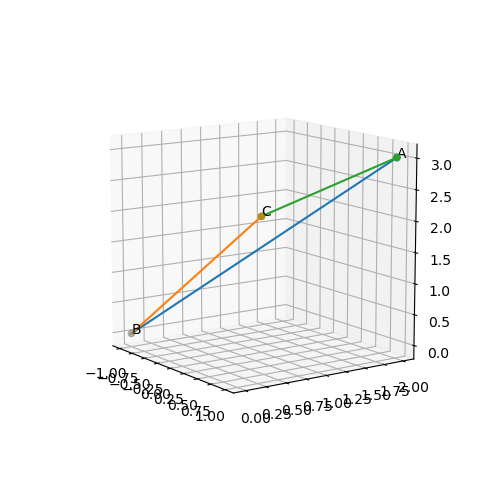
\includegraphics[width=\linewidth]{figs/Figure_1.png}
   \caption{Triangle ABC}
   \label{fig:TriangleABC}
\end{figure}

\end{document}


\fi

\item If $\vec{a}=\vec{b}+\vec{c}$, then is it true that $|\vec{a}|=|\vec{b}|+|\vec{c}|$? Justify your answer.\\
	\solution
		\iffalse
\documentclass[journal,12pt,twocolumn]{IEEEtran}
\usepackage{graphicx}
\graphicspath{{./figs/}}{}
\usepackage{amsmath,amssymb,amsfonts,amsthm}
\newcommand{\myvec}[1]{\ensuremath{\begin{pmatrix}#1\end{pmatrix}}}
\providecommand{\norm}[1]{\lVert#1\rVert}
\usepackage{listings}
\usepackage{watermark}
\usepackage{titlesec}
\usepackage{caption}
\newcommand{\mydet}[1]{\ensuremath{\begin{vmatrix}#1\end{vmatrix}}}
\let\vec\mathbf
\lstset{
frame=single, 
breaklines=true,
columns=fullflexible
}
\thiswatermark{\centering \put(0,-105.0){
\includegraphics[scale=0.15]{/sdcard/IITH/vectors/12.10.5.4/figs/logo.png}} }
\title{\mytitle}
\title{
Assignment - 12.10.5.4
}
\author{Surajit Sarkar}
\begin{document}
\maketitle
\tableofcontents
\bigskip
\section{\textbf{Problem}}
if $\vec{a}=\vec{b}+\vec{c}$, then is true that $|\vec{a}|=|\vec{b}|+|\vec{c}|$?
Justify your answer .
\section{\textbf{Solution}}
Given
\begin{align}
    \vec{a}=\vec{b}+\vec{c}
\end{align}
\fi
Let
\begin{align}
    \vec{b}=\myvec{1\\2\\3},\vec{c}=\myvec{2\\-1\\-2}
\end{align}
Then
\begin{align}
	\vec{a}&=\vec{b}+\vec{c}
    =\myvec{3\\1\\1}
    \\
	\implies
    \norm{\vec{a}}
    &=\sqrt{11},\,
    \norm{\vec{b}}    =\sqrt{14},\,
    \norm{\vec{c}}
    =3.
\end{align}
Thus
\begin{align}
	\norm{\vec{a}}\ne\norm{\vec{b}}+\norm{\vec{c}}
\end{align}


\item Find the value of x for which $x(\hat{i}+\hat{j}+\hat{k})$ is a unit vector.\\
	\solution
		\iffalse
\documentclass[12pt]{article}
\usepackage{graphicx}
\usepackage[none]{hyphenat}
\usepackage{graphicx}
\usepackage{listings}
\usepackage[english]{babel}
\usepackage{graphicx}
\usepackage{caption} 
\usepackage{booktabs}
\usepackage{array}
\usepackage{amssymb} % for \because
\usepackage{amsmath}   % for having text in math mode
\usepackage{extarrows} % for Row operations arrows
\usepackage{listings}
\lstset{
  frame=single,
  breaklines=true
}
\usepackage{hyperref}
  
%Following 2 lines were added to remove the blank page at the beginning
\usepackage{atbegshi}% http://ctan.org/pkg/atbegshi
\AtBeginDocument{\AtBeginShipoutNext{\AtBeginShipoutDiscard}}


%New macro definitions
\newcommand{\mydet}[1]{\ensuremath{\begin{vmatrix}#1\end{vmatrix}}}
\providecommand{\brak}[1]{\ensuremath{\left(#1\right)}}
\providecommand{\norm}[1]{\left\lVert#1\right\rVert}
\newcommand{\solution}{\noindent \textbf{Solution: }}
\newcommand{\myvec}[1]{\ensuremath{\begin{pmatrix}#1\end{pmatrix}}}
\providecommand{\abs}[1]{\left\vert#1\right\vert}
\let\vec\mathbf

\begin{document}

\begin{center}
\title{\textbf{Equation  of Unit Vector}}
\date{\vspace{-5ex}} %Not to print date automatically
\maketitle
\end{center}
\setcounter{page}{1}
\section{12$^{th}$ Maths - Chapter 10}
\textbf{This is Problem-5 from Exercise 5.5}
\begin{enumerate}
\item Find the value of $x$ for which $x(\hat{i}+\hat{j}+\hat{k})$ is a unit vector
\section{Solution}
\solution
\fi
Let
\begin{align} 
\vec{x}&=x\myvec{1\\1\\1}
\implies
\norm{\vec{x}}=1
\\
\implies 
x\sqrt{3}&=1,\,
	\text{or, }x=\frac{1}{\sqrt{3}}
\end{align}   

\end{enumerate}
